\documentclass[twoside]{book}

% Packages required by doxygen
\usepackage{fixltx2e}
\usepackage{calc}
\usepackage{doxygen}
\usepackage[export]{adjustbox} % also loads graphicx
\usepackage{graphicx}
\usepackage[utf8]{inputenc}
\usepackage{makeidx}
\usepackage{multicol}
\usepackage{multirow}
\PassOptionsToPackage{warn}{textcomp}
\usepackage{textcomp}
\usepackage[nointegrals]{wasysym}
\usepackage[table]{xcolor}

% Font selection
\usepackage[T1]{fontenc}
\usepackage[scaled=.90]{helvet}
\usepackage{courier}
\usepackage{amssymb}
\usepackage{sectsty}
\renewcommand{\familydefault}{\sfdefault}
\allsectionsfont{%
  \fontseries{bc}\selectfont%
  \color{darkgray}%
}
\renewcommand{\DoxyLabelFont}{%
  \fontseries{bc}\selectfont%
  \color{darkgray}%
}
\newcommand{\+}{\discretionary{\mbox{\scriptsize$\hookleftarrow$}}{}{}}

% Page & text layout
\usepackage{geometry}
\geometry{%
  a4paper,%
  top=2.5cm,%
  bottom=2.5cm,%
  left=2.5cm,%
  right=2.5cm%
}
\tolerance=750
\hfuzz=15pt
\hbadness=750
\setlength{\emergencystretch}{15pt}
\setlength{\parindent}{0cm}
\setlength{\parskip}{3ex plus 2ex minus 2ex}
\makeatletter
\renewcommand{\paragraph}{%
  \@startsection{paragraph}{4}{0ex}{-1.0ex}{1.0ex}{%
    \normalfont\normalsize\bfseries\SS@parafont%
  }%
}
\renewcommand{\subparagraph}{%
  \@startsection{subparagraph}{5}{0ex}{-1.0ex}{1.0ex}{%
    \normalfont\normalsize\bfseries\SS@subparafont%
  }%
}
\makeatother

% Headers & footers
\usepackage{fancyhdr}
\pagestyle{fancyplain}
\fancyhead[LE]{\fancyplain{}{\bfseries\thepage}}
\fancyhead[CE]{\fancyplain{}{}}
\fancyhead[RE]{\fancyplain{}{\bfseries\leftmark}}
\fancyhead[LO]{\fancyplain{}{\bfseries\rightmark}}
\fancyhead[CO]{\fancyplain{}{}}
\fancyhead[RO]{\fancyplain{}{\bfseries\thepage}}
\fancyfoot[LE]{\fancyplain{}{}}
\fancyfoot[CE]{\fancyplain{}{}}
\fancyfoot[RE]{\fancyplain{}{\bfseries\scriptsize Generated by Doxygen }}
\fancyfoot[LO]{\fancyplain{}{\bfseries\scriptsize Generated by Doxygen }}
\fancyfoot[CO]{\fancyplain{}{}}
\fancyfoot[RO]{\fancyplain{}{}}
\renewcommand{\footrulewidth}{0.4pt}
\renewcommand{\chaptermark}[1]{%
  \markboth{#1}{}%
}
\renewcommand{\sectionmark}[1]{%
  \markright{\thesection\ #1}%
}

% Indices & bibliography
\usepackage{natbib}
\usepackage[titles]{tocloft}
\setcounter{tocdepth}{3}
\setcounter{secnumdepth}{5}
\makeindex

% Hyperlinks (required, but should be loaded last)
\usepackage{ifpdf}
\ifpdf
  \usepackage[pdftex,pagebackref=true]{hyperref}
\else
  \usepackage[ps2pdf,pagebackref=true]{hyperref}
\fi
\hypersetup{%
  colorlinks=true,%
  linkcolor=blue,%
  citecolor=blue,%
  unicode%
}

% Custom commands
\newcommand{\clearemptydoublepage}{%
  \newpage{\pagestyle{empty}\cleardoublepage}%
}

\usepackage{caption}
\captionsetup{labelsep=space,justification=centering,font={bf},singlelinecheck=off,skip=4pt,position=top}

%===== C O N T E N T S =====

\begin{document}

% Titlepage & ToC
\hypersetup{pageanchor=false,
             bookmarksnumbered=true,
             pdfencoding=unicode
            }
\pagenumbering{alph}
\begin{titlepage}
\vspace*{7cm}
\begin{center}%
{\Large spmv }\\
\vspace*{1cm}
{\large Generated by Doxygen 1.8.13}\\
\end{center}
\end{titlepage}
\clearemptydoublepage
\pagenumbering{roman}
\tableofcontents
\clearemptydoublepage
\pagenumbering{arabic}
\hypersetup{pageanchor=true}

%--- Begin generated contents ---
\chapter{Class Index}
\section{Class List}
Here are the classes, structs, unions and interfaces with brief descriptions\+:\begin{DoxyCompactList}
\item\contentsline{section}{\hyperlink{structcmdline__options__t}{cmdline\+\_\+options\+\_\+t} \\*Command line option }{\pageref{structcmdline__options__t}}{}
\item\contentsline{section}{\hyperlink{structcoo__elem__t}{coo\+\_\+elem\+\_\+t} \\*Element of coordinate list (i, j, a) }{\pageref{structcoo__elem__t}}{}
\item\contentsline{section}{\hyperlink{structcoo__t}{coo\+\_\+t} \\*Sparse matrix in coodinate list format }{\pageref{structcoo__t}}{}
\item\contentsline{section}{\hyperlink{structcsr__elem__t}{csr\+\_\+elem\+\_\+t} \\*Element of compressed sparse row }{\pageref{structcsr__elem__t}}{}
\item\contentsline{section}{\hyperlink{structcsr__t}{csr\+\_\+t} \\*Sparse matrix in compressed row format }{\pageref{structcsr__t}}{}
\item\contentsline{section}{\hyperlink{structidx__pair__t}{idx\+\_\+pair\+\_\+t} \\*Pair of two indices (i and j) }{\pageref{structidx__pair__t}}{}
\item\contentsline{section}{\hyperlink{structimage__t}{image\+\_\+t} \\*Data structure through which to convert a matrix into a gnuplot file }{\pageref{structimage__t}}{}
\item\contentsline{section}{\hyperlink{structsparse__format__table__entry__t}{sparse\+\_\+format\+\_\+table\+\_\+entry\+\_\+t} \\*Pair of the index value (sparse\+\_\+format\+\_\+t) and its name }{\pageref{structsparse__format__table__entry__t}}{}
\item\contentsline{section}{\hyperlink{structsparse__format__table__t}{sparse\+\_\+format\+\_\+table\+\_\+t} \\*Table of sparse format and their names }{\pageref{structsparse__format__table__t}}{}
\item\contentsline{section}{\hyperlink{structsparse__matrix__type__table__entry__t}{sparse\+\_\+matrix\+\_\+type\+\_\+table\+\_\+entry\+\_\+t} \\*Pair of the index value (matrix\+\_\+type\+\_\+t) and its name }{\pageref{structsparse__matrix__type__table__entry__t}}{}
\item\contentsline{section}{\hyperlink{structsparse__matrix__type__table__t}{sparse\+\_\+matrix\+\_\+type\+\_\+table\+\_\+t} \\*Table of sparse matrix types and their names }{\pageref{structsparse__matrix__type__table__t}}{}
\item\contentsline{section}{\hyperlink{structsparse__t}{sparse\+\_\+t} \\*Sparse matrix (in any format) }{\pageref{structsparse__t}}{}
\item\contentsline{section}{\hyperlink{structspmv__algo__table__entry__t}{spmv\+\_\+algo\+\_\+table\+\_\+entry\+\_\+t} \\*Pair of the index value (spmv\+\_\+algo\+\_\+t) and its name }{\pageref{structspmv__algo__table__entry__t}}{}
\item\contentsline{section}{\hyperlink{structspmv__algo__table__t}{spmv\+\_\+algo\+\_\+table\+\_\+t} \\*Table of spmv algorithms and their names }{\pageref{structspmv__algo__table__t}}{}
\item\contentsline{section}{\hyperlink{structvec__t}{vec\+\_\+t} \\*Vector }{\pageref{structvec__t}}{}
\end{DoxyCompactList}

\chapter{File Index}
\section{File List}
Here is a list of all documented files with brief descriptions\+:\begin{DoxyCompactList}
\item\contentsline{section}{/home/tau/public\+\_\+html/lecture/parallel\+\_\+distributed/2018/parallel-\/distributed-\/handson/03spmv/\hyperlink{cuda__util_8h}{cuda\+\_\+util.\+h} \\*Small utility functions for cuda }{\pageref{cuda__util_8h}}{}
\item\contentsline{section}{/home/tau/public\+\_\+html/lecture/parallel\+\_\+distributed/2018/parallel-\/distributed-\/handson/03spmv/\hyperlink{spmv_8cc}{spmv.\+cc} \\*Sparse matrix vector multiplication }{\pageref{spmv_8cc}}{}
\end{DoxyCompactList}

\chapter{Class Documentation}
\hypertarget{structcmdline__options__t}{}\section{cmdline\+\_\+options\+\_\+t Struct Reference}
\label{structcmdline__options__t}\index{cmdline\+\_\+options\+\_\+t@{cmdline\+\_\+options\+\_\+t}}


command line option  


\subsection*{Public Attributes}
\begin{DoxyCompactItemize}
\item 
\hyperlink{spmv_8cc_a8e93478a00e685bea5e6a3f617bf03a3}{idx\+\_\+t} \hyperlink{structcmdline__options__t_aeb40f98dbcd53dc727b1d7dbb566924f}{M}
\item 
\hyperlink{spmv_8cc_a8e93478a00e685bea5e6a3f617bf03a3}{idx\+\_\+t} \hyperlink{structcmdline__options__t_aa58f87808071259b5aa8f17c64bf2960}{N}
\item 
\hyperlink{spmv_8cc_a8e93478a00e685bea5e6a3f617bf03a3}{idx\+\_\+t} \hyperlink{structcmdline__options__t_aec8f7846348926cda6d62023f62d0d25}{nnz}
\item 
long \hyperlink{structcmdline__options__t_acb60cada2976487316be88bf4309e7d6}{repeat}
\item 
char $\ast$ \hyperlink{structcmdline__options__t_a16fe2748dfda1fc639d7e3321eb0e4a9}{format\+\_\+str}
\item 
\hyperlink{spmv_8cc_a8c0094893526c01b430903b2d9227256}{sparse\+\_\+format\+\_\+t} \hyperlink{structcmdline__options__t_af8a99d8cdebe0bc5fd512d2254727231}{format}
\item 
char $\ast$ \hyperlink{structcmdline__options__t_a1669264b4602341b949007ca4336dfc2}{matrix\+\_\+type\+\_\+str}
\item 
\hyperlink{spmv_8cc_a43a568fb26bc32aeaad07769cc524c45}{sparse\+\_\+matrix\+\_\+type\+\_\+t} \hyperlink{structcmdline__options__t_abc77475ac02e2e93b9f978ea22cb6244}{matrix\+\_\+type}
\item 
char $\ast$ \hyperlink{structcmdline__options__t_ae8ab407cdc87a30c1b4cdf6b424c8370}{algo\+\_\+str}
\item 
\hyperlink{spmv_8cc_ad2cf0493af54bf76c5be68b4634fcab7}{spmv\+\_\+algo\+\_\+t} \hyperlink{structcmdline__options__t_afddf83f65e6e4a14761d84a5e876e6ac}{algo}
\item 
char $\ast$ \hyperlink{structcmdline__options__t_a2db02208284cd9664c88e6f0e7140d6d}{coo\+\_\+file}
\item 
char $\ast$ \hyperlink{structcmdline__options__t_a4ae2cfd5fda7a25e302fff37c1201f93}{rmat\+\_\+str}
\item 
double \hyperlink{structcmdline__options__t_a60e05c62d3fd439c03fd26d9f8078a4b}{rmat} \mbox{[}2\mbox{]}\mbox{[}2\mbox{]}
\item 
char $\ast$ \hyperlink{structcmdline__options__t_aa4b96337328846dd1d2c0ca8eee7933f}{dump}
\item 
\hyperlink{spmv_8cc_a8e93478a00e685bea5e6a3f617bf03a3}{idx\+\_\+t} \hyperlink{structcmdline__options__t_ad1c5aa9c8877bae151ca40373f68a848}{img\+\_\+W}
\item 
\hyperlink{spmv_8cc_a8e93478a00e685bea5e6a3f617bf03a3}{idx\+\_\+t} \hyperlink{structcmdline__options__t_a463c33340772fb1baf377fb67f3d7a40}{img\+\_\+H}
\item 
long \hyperlink{structcmdline__options__t_a065412d7cdc54cdae630389c3fda266e}{seed}
\item 
int \hyperlink{structcmdline__options__t_a25f9087b240da0b93a4295fa5f173c88}{error}
\item 
int \hyperlink{structcmdline__options__t_ab02741e43bb19900e87caaec3a8dd794}{help}
\end{DoxyCompactItemize}


\subsection{Detailed Description}
command line option 

\subsection{Member Data Documentation}
\mbox{\Hypertarget{structcmdline__options__t_afddf83f65e6e4a14761d84a5e876e6ac}\label{structcmdline__options__t_afddf83f65e6e4a14761d84a5e876e6ac}} 
\index{cmdline\+\_\+options\+\_\+t@{cmdline\+\_\+options\+\_\+t}!algo@{algo}}
\index{algo@{algo}!cmdline\+\_\+options\+\_\+t@{cmdline\+\_\+options\+\_\+t}}
\subsubsection{\texorpdfstring{algo}{algo}}
{\footnotesize\ttfamily \hyperlink{spmv_8cc_ad2cf0493af54bf76c5be68b4634fcab7}{spmv\+\_\+algo\+\_\+t} cmdline\+\_\+options\+\_\+t\+::algo}

algo\+\_\+str converted to enum \mbox{\Hypertarget{structcmdline__options__t_ae8ab407cdc87a30c1b4cdf6b424c8370}\label{structcmdline__options__t_ae8ab407cdc87a30c1b4cdf6b424c8370}} 
\index{cmdline\+\_\+options\+\_\+t@{cmdline\+\_\+options\+\_\+t}!algo\+\_\+str@{algo\+\_\+str}}
\index{algo\+\_\+str@{algo\+\_\+str}!cmdline\+\_\+options\+\_\+t@{cmdline\+\_\+options\+\_\+t}}
\subsubsection{\texorpdfstring{algo\+\_\+str}{algo\_str}}
{\footnotesize\ttfamily char$\ast$ cmdline\+\_\+options\+\_\+t\+::algo\+\_\+str}

algorithm string (serial, parallel, cuda) \mbox{\Hypertarget{structcmdline__options__t_a2db02208284cd9664c88e6f0e7140d6d}\label{structcmdline__options__t_a2db02208284cd9664c88e6f0e7140d6d}} 
\index{cmdline\+\_\+options\+\_\+t@{cmdline\+\_\+options\+\_\+t}!coo\+\_\+file@{coo\+\_\+file}}
\index{coo\+\_\+file@{coo\+\_\+file}!cmdline\+\_\+options\+\_\+t@{cmdline\+\_\+options\+\_\+t}}
\subsubsection{\texorpdfstring{coo\+\_\+file}{coo\_file}}
{\footnotesize\ttfamily char$\ast$ cmdline\+\_\+options\+\_\+t\+::coo\+\_\+file}

file \mbox{\Hypertarget{structcmdline__options__t_aa4b96337328846dd1d2c0ca8eee7933f}\label{structcmdline__options__t_aa4b96337328846dd1d2c0ca8eee7933f}} 
\index{cmdline\+\_\+options\+\_\+t@{cmdline\+\_\+options\+\_\+t}!dump@{dump}}
\index{dump@{dump}!cmdline\+\_\+options\+\_\+t@{cmdline\+\_\+options\+\_\+t}}
\subsubsection{\texorpdfstring{dump}{dump}}
{\footnotesize\ttfamily char$\ast$ cmdline\+\_\+options\+\_\+t\+::dump}

file name to dump image (gnuplot) data \mbox{\Hypertarget{structcmdline__options__t_a25f9087b240da0b93a4295fa5f173c88}\label{structcmdline__options__t_a25f9087b240da0b93a4295fa5f173c88}} 
\index{cmdline\+\_\+options\+\_\+t@{cmdline\+\_\+options\+\_\+t}!error@{error}}
\index{error@{error}!cmdline\+\_\+options\+\_\+t@{cmdline\+\_\+options\+\_\+t}}
\subsubsection{\texorpdfstring{error}{error}}
{\footnotesize\ttfamily int cmdline\+\_\+options\+\_\+t\+::error}

set when we encounter an error \mbox{\Hypertarget{structcmdline__options__t_af8a99d8cdebe0bc5fd512d2254727231}\label{structcmdline__options__t_af8a99d8cdebe0bc5fd512d2254727231}} 
\index{cmdline\+\_\+options\+\_\+t@{cmdline\+\_\+options\+\_\+t}!format@{format}}
\index{format@{format}!cmdline\+\_\+options\+\_\+t@{cmdline\+\_\+options\+\_\+t}}
\subsubsection{\texorpdfstring{format}{format}}
{\footnotesize\ttfamily \hyperlink{spmv_8cc_a8c0094893526c01b430903b2d9227256}{sparse\+\_\+format\+\_\+t} cmdline\+\_\+options\+\_\+t\+::format}

format\+\_\+str converted to enum \mbox{\Hypertarget{structcmdline__options__t_a16fe2748dfda1fc639d7e3321eb0e4a9}\label{structcmdline__options__t_a16fe2748dfda1fc639d7e3321eb0e4a9}} 
\index{cmdline\+\_\+options\+\_\+t@{cmdline\+\_\+options\+\_\+t}!format\+\_\+str@{format\+\_\+str}}
\index{format\+\_\+str@{format\+\_\+str}!cmdline\+\_\+options\+\_\+t@{cmdline\+\_\+options\+\_\+t}}
\subsubsection{\texorpdfstring{format\+\_\+str}{format\_str}}
{\footnotesize\ttfamily char$\ast$ cmdline\+\_\+options\+\_\+t\+::format\+\_\+str}

format string (coo, coo\+\_\+sorted, csr) \mbox{\Hypertarget{structcmdline__options__t_ab02741e43bb19900e87caaec3a8dd794}\label{structcmdline__options__t_ab02741e43bb19900e87caaec3a8dd794}} 
\index{cmdline\+\_\+options\+\_\+t@{cmdline\+\_\+options\+\_\+t}!help@{help}}
\index{help@{help}!cmdline\+\_\+options\+\_\+t@{cmdline\+\_\+options\+\_\+t}}
\subsubsection{\texorpdfstring{help}{help}}
{\footnotesize\ttfamily int cmdline\+\_\+options\+\_\+t\+::help}

set when -\/h / --help is given \mbox{\Hypertarget{structcmdline__options__t_a463c33340772fb1baf377fb67f3d7a40}\label{structcmdline__options__t_a463c33340772fb1baf377fb67f3d7a40}} 
\index{cmdline\+\_\+options\+\_\+t@{cmdline\+\_\+options\+\_\+t}!img\+\_\+H@{img\+\_\+H}}
\index{img\+\_\+H@{img\+\_\+H}!cmdline\+\_\+options\+\_\+t@{cmdline\+\_\+options\+\_\+t}}
\subsubsection{\texorpdfstring{img\+\_\+H}{img\_H}}
{\footnotesize\ttfamily \hyperlink{spmv_8cc_a8e93478a00e685bea5e6a3f617bf03a3}{idx\+\_\+t} cmdline\+\_\+options\+\_\+t\+::img\+\_\+H}

height of the dumped image \mbox{\Hypertarget{structcmdline__options__t_ad1c5aa9c8877bae151ca40373f68a848}\label{structcmdline__options__t_ad1c5aa9c8877bae151ca40373f68a848}} 
\index{cmdline\+\_\+options\+\_\+t@{cmdline\+\_\+options\+\_\+t}!img\+\_\+W@{img\+\_\+W}}
\index{img\+\_\+W@{img\+\_\+W}!cmdline\+\_\+options\+\_\+t@{cmdline\+\_\+options\+\_\+t}}
\subsubsection{\texorpdfstring{img\+\_\+W}{img\_W}}
{\footnotesize\ttfamily \hyperlink{spmv_8cc_a8e93478a00e685bea5e6a3f617bf03a3}{idx\+\_\+t} cmdline\+\_\+options\+\_\+t\+::img\+\_\+W}

width of the dumped image \mbox{\Hypertarget{structcmdline__options__t_aeb40f98dbcd53dc727b1d7dbb566924f}\label{structcmdline__options__t_aeb40f98dbcd53dc727b1d7dbb566924f}} 
\index{cmdline\+\_\+options\+\_\+t@{cmdline\+\_\+options\+\_\+t}!M@{M}}
\index{M@{M}!cmdline\+\_\+options\+\_\+t@{cmdline\+\_\+options\+\_\+t}}
\subsubsection{\texorpdfstring{M}{M}}
{\footnotesize\ttfamily \hyperlink{spmv_8cc_a8e93478a00e685bea5e6a3f617bf03a3}{idx\+\_\+t} cmdline\+\_\+options\+\_\+t\+::M}

number of rows \mbox{\Hypertarget{structcmdline__options__t_abc77475ac02e2e93b9f978ea22cb6244}\label{structcmdline__options__t_abc77475ac02e2e93b9f978ea22cb6244}} 
\index{cmdline\+\_\+options\+\_\+t@{cmdline\+\_\+options\+\_\+t}!matrix\+\_\+type@{matrix\+\_\+type}}
\index{matrix\+\_\+type@{matrix\+\_\+type}!cmdline\+\_\+options\+\_\+t@{cmdline\+\_\+options\+\_\+t}}
\subsubsection{\texorpdfstring{matrix\+\_\+type}{matrix\_type}}
{\footnotesize\ttfamily \hyperlink{spmv_8cc_a43a568fb26bc32aeaad07769cc524c45}{sparse\+\_\+matrix\+\_\+type\+\_\+t} cmdline\+\_\+options\+\_\+t\+::matrix\+\_\+type}

matrix\+\_\+type\+\_\+str converted to enum \mbox{\Hypertarget{structcmdline__options__t_a1669264b4602341b949007ca4336dfc2}\label{structcmdline__options__t_a1669264b4602341b949007ca4336dfc2}} 
\index{cmdline\+\_\+options\+\_\+t@{cmdline\+\_\+options\+\_\+t}!matrix\+\_\+type\+\_\+str@{matrix\+\_\+type\+\_\+str}}
\index{matrix\+\_\+type\+\_\+str@{matrix\+\_\+type\+\_\+str}!cmdline\+\_\+options\+\_\+t@{cmdline\+\_\+options\+\_\+t}}
\subsubsection{\texorpdfstring{matrix\+\_\+type\+\_\+str}{matrix\_type\_str}}
{\footnotesize\ttfamily char$\ast$ cmdline\+\_\+options\+\_\+t\+::matrix\+\_\+type\+\_\+str}

matrix type (random, rmat, file) \mbox{\Hypertarget{structcmdline__options__t_aa58f87808071259b5aa8f17c64bf2960}\label{structcmdline__options__t_aa58f87808071259b5aa8f17c64bf2960}} 
\index{cmdline\+\_\+options\+\_\+t@{cmdline\+\_\+options\+\_\+t}!N@{N}}
\index{N@{N}!cmdline\+\_\+options\+\_\+t@{cmdline\+\_\+options\+\_\+t}}
\subsubsection{\texorpdfstring{N}{N}}
{\footnotesize\ttfamily \hyperlink{spmv_8cc_a8e93478a00e685bea5e6a3f617bf03a3}{idx\+\_\+t} cmdline\+\_\+options\+\_\+t\+::N}

number of columns \mbox{\Hypertarget{structcmdline__options__t_aec8f7846348926cda6d62023f62d0d25}\label{structcmdline__options__t_aec8f7846348926cda6d62023f62d0d25}} 
\index{cmdline\+\_\+options\+\_\+t@{cmdline\+\_\+options\+\_\+t}!nnz@{nnz}}
\index{nnz@{nnz}!cmdline\+\_\+options\+\_\+t@{cmdline\+\_\+options\+\_\+t}}
\subsubsection{\texorpdfstring{nnz}{nnz}}
{\footnotesize\ttfamily \hyperlink{spmv_8cc_a8e93478a00e685bea5e6a3f617bf03a3}{idx\+\_\+t} cmdline\+\_\+options\+\_\+t\+::nnz}

number of non-\/zero elements \mbox{\Hypertarget{structcmdline__options__t_acb60cada2976487316be88bf4309e7d6}\label{structcmdline__options__t_acb60cada2976487316be88bf4309e7d6}} 
\index{cmdline\+\_\+options\+\_\+t@{cmdline\+\_\+options\+\_\+t}!repeat@{repeat}}
\index{repeat@{repeat}!cmdline\+\_\+options\+\_\+t@{cmdline\+\_\+options\+\_\+t}}
\subsubsection{\texorpdfstring{repeat}{repeat}}
{\footnotesize\ttfamily long cmdline\+\_\+options\+\_\+t\+::repeat}

number of iterations (tA (Ax)) \mbox{\Hypertarget{structcmdline__options__t_a60e05c62d3fd439c03fd26d9f8078a4b}\label{structcmdline__options__t_a60e05c62d3fd439c03fd26d9f8078a4b}} 
\index{cmdline\+\_\+options\+\_\+t@{cmdline\+\_\+options\+\_\+t}!rmat@{rmat}}
\index{rmat@{rmat}!cmdline\+\_\+options\+\_\+t@{cmdline\+\_\+options\+\_\+t}}
\subsubsection{\texorpdfstring{rmat}{rmat}}
{\footnotesize\ttfamily double cmdline\+\_\+options\+\_\+t\+::rmat\mbox{[}2\mbox{]}\mbox{[}2\mbox{]}}

\{ \{ a, b \}, \{ c, d \} \} probability of rmat \mbox{\Hypertarget{structcmdline__options__t_a4ae2cfd5fda7a25e302fff37c1201f93}\label{structcmdline__options__t_a4ae2cfd5fda7a25e302fff37c1201f93}} 
\index{cmdline\+\_\+options\+\_\+t@{cmdline\+\_\+options\+\_\+t}!rmat\+\_\+str@{rmat\+\_\+str}}
\index{rmat\+\_\+str@{rmat\+\_\+str}!cmdline\+\_\+options\+\_\+t@{cmdline\+\_\+options\+\_\+t}}
\subsubsection{\texorpdfstring{rmat\+\_\+str}{rmat\_str}}
{\footnotesize\ttfamily char$\ast$ cmdline\+\_\+options\+\_\+t\+::rmat\+\_\+str}

a,b,c,d probability of rmat \mbox{\Hypertarget{structcmdline__options__t_a065412d7cdc54cdae630389c3fda266e}\label{structcmdline__options__t_a065412d7cdc54cdae630389c3fda266e}} 
\index{cmdline\+\_\+options\+\_\+t@{cmdline\+\_\+options\+\_\+t}!seed@{seed}}
\index{seed@{seed}!cmdline\+\_\+options\+\_\+t@{cmdline\+\_\+options\+\_\+t}}
\subsubsection{\texorpdfstring{seed}{seed}}
{\footnotesize\ttfamily long cmdline\+\_\+options\+\_\+t\+::seed}

random number generator seed 

The documentation for this struct was generated from the following file\+:\begin{DoxyCompactItemize}
\item 
/home/tau/public\+\_\+html/lecture/parallel\+\_\+distributed/2018/parallel-\/distributed-\/handson/03spmv/\hyperlink{spmv_8cc}{spmv.\+cc}\end{DoxyCompactItemize}

\hypertarget{structcoo__elem__t}{}\section{coo\+\_\+elem\+\_\+t Struct Reference}
\label{structcoo__elem__t}\index{coo\+\_\+elem\+\_\+t@{coo\+\_\+elem\+\_\+t}}


an element of coordinate list (i, j, a)  


\subsection*{Public Attributes}
\begin{DoxyCompactItemize}
\item 
\hyperlink{spmv_8cc_a8e93478a00e685bea5e6a3f617bf03a3}{idx\+\_\+t} \hyperlink{structcoo__elem__t_a4bba7fd2cc28e3a6dd2eea0fed6b5a06}{i}
\item 
\hyperlink{spmv_8cc_a8e93478a00e685bea5e6a3f617bf03a3}{idx\+\_\+t} \hyperlink{structcoo__elem__t_a45a4cd1c7ffe70ddd75dff7c764bbfc6}{j}
\item 
\hyperlink{spmv_8cc_a11d147c64891830c9e79b3315b1b2e21}{real} \hyperlink{structcoo__elem__t_ad835f42450aaf40546d685fdfe1f9fcf}{a}
\end{DoxyCompactItemize}


\subsection{Detailed Description}
an element of coordinate list (i, j, a) 

\subsection{Member Data Documentation}
\mbox{\Hypertarget{structcoo__elem__t_ad835f42450aaf40546d685fdfe1f9fcf}\label{structcoo__elem__t_ad835f42450aaf40546d685fdfe1f9fcf}} 
\index{coo\+\_\+elem\+\_\+t@{coo\+\_\+elem\+\_\+t}!a@{a}}
\index{a@{a}!coo\+\_\+elem\+\_\+t@{coo\+\_\+elem\+\_\+t}}
\subsubsection{\texorpdfstring{a}{a}}
{\footnotesize\ttfamily \hyperlink{spmv_8cc_a11d147c64891830c9e79b3315b1b2e21}{real} coo\+\_\+elem\+\_\+t\+::a}

element \mbox{\Hypertarget{structcoo__elem__t_a4bba7fd2cc28e3a6dd2eea0fed6b5a06}\label{structcoo__elem__t_a4bba7fd2cc28e3a6dd2eea0fed6b5a06}} 
\index{coo\+\_\+elem\+\_\+t@{coo\+\_\+elem\+\_\+t}!i@{i}}
\index{i@{i}!coo\+\_\+elem\+\_\+t@{coo\+\_\+elem\+\_\+t}}
\subsubsection{\texorpdfstring{i}{i}}
{\footnotesize\ttfamily \hyperlink{spmv_8cc_a8e93478a00e685bea5e6a3f617bf03a3}{idx\+\_\+t} coo\+\_\+elem\+\_\+t\+::i}

row \mbox{\Hypertarget{structcoo__elem__t_a45a4cd1c7ffe70ddd75dff7c764bbfc6}\label{structcoo__elem__t_a45a4cd1c7ffe70ddd75dff7c764bbfc6}} 
\index{coo\+\_\+elem\+\_\+t@{coo\+\_\+elem\+\_\+t}!j@{j}}
\index{j@{j}!coo\+\_\+elem\+\_\+t@{coo\+\_\+elem\+\_\+t}}
\subsubsection{\texorpdfstring{j}{j}}
{\footnotesize\ttfamily \hyperlink{spmv_8cc_a8e93478a00e685bea5e6a3f617bf03a3}{idx\+\_\+t} coo\+\_\+elem\+\_\+t\+::j}

column 

The documentation for this struct was generated from the following file\+:\begin{DoxyCompactItemize}
\item 
/home/tau/public\+\_\+html/lecture/parallel\+\_\+distributed/2018/ex/00spmv/\hyperlink{spmv_8cc}{spmv.\+cc}\end{DoxyCompactItemize}

\hypertarget{structcoo__t}{}\section{coo\+\_\+t Struct Reference}
\label{structcoo__t}\index{coo\+\_\+t@{coo\+\_\+t}}


sparse matrix in coodinate list format  




Collaboration diagram for coo\+\_\+t\+:\nopagebreak
\begin{figure}[H]
\begin{center}
\leavevmode
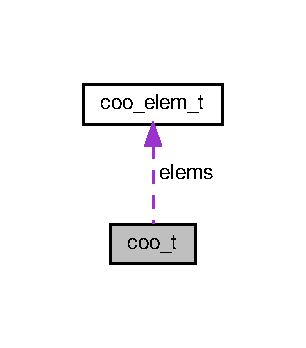
\includegraphics[width=147pt]{structcoo__t__coll__graph}
\end{center}
\end{figure}
\subsection*{Public Attributes}
\begin{DoxyCompactItemize}
\item 
\hyperlink{structcoo__elem__t}{coo\+\_\+elem\+\_\+t} $\ast$ \hyperlink{structcoo__t_a3e74f1e3dadd34e5439f859fab277b54}{elems}
\end{DoxyCompactItemize}


\subsection{Detailed Description}
sparse matrix in coodinate list format 

\subsection{Member Data Documentation}
\mbox{\Hypertarget{structcoo__t_a3e74f1e3dadd34e5439f859fab277b54}\label{structcoo__t_a3e74f1e3dadd34e5439f859fab277b54}} 
\index{coo\+\_\+t@{coo\+\_\+t}!elems@{elems}}
\index{elems@{elems}!coo\+\_\+t@{coo\+\_\+t}}
\subsubsection{\texorpdfstring{elems}{elems}}
{\footnotesize\ttfamily \hyperlink{structcoo__elem__t}{coo\+\_\+elem\+\_\+t}$\ast$ coo\+\_\+t\+::elems}

elements array 

The documentation for this struct was generated from the following file\+:\begin{DoxyCompactItemize}
\item 
/home/tau/public\+\_\+html/lecture/parallel\+\_\+distributed/2018/handson/tau/parallel-\/distributed-\/handson/03spmv/\hyperlink{spmv_8cc}{spmv.\+cc}\end{DoxyCompactItemize}

\hypertarget{structcsr__elem__t}{}\section{csr\+\_\+elem\+\_\+t Struct Reference}
\label{structcsr__elem__t}\index{csr\+\_\+elem\+\_\+t@{csr\+\_\+elem\+\_\+t}}


an element of compressed sparse row  


\subsection*{Public Attributes}
\begin{DoxyCompactItemize}
\item 
\hyperlink{spmv_8cc_a8e93478a00e685bea5e6a3f617bf03a3}{idx\+\_\+t} \hyperlink{structcsr__elem__t_a4525598ab26d6263b2242cc33511ca7f}{j}
\item 
\hyperlink{spmv_8cc_a11d147c64891830c9e79b3315b1b2e21}{real} \hyperlink{structcsr__elem__t_a55e480eefa495ee8b6e359a5f5a94a4f}{a}
\end{DoxyCompactItemize}


\subsection{Detailed Description}
an element of compressed sparse row 

\subsection{Member Data Documentation}
\mbox{\Hypertarget{structcsr__elem__t_a55e480eefa495ee8b6e359a5f5a94a4f}\label{structcsr__elem__t_a55e480eefa495ee8b6e359a5f5a94a4f}} 
\index{csr\+\_\+elem\+\_\+t@{csr\+\_\+elem\+\_\+t}!a@{a}}
\index{a@{a}!csr\+\_\+elem\+\_\+t@{csr\+\_\+elem\+\_\+t}}
\subsubsection{\texorpdfstring{a}{a}}
{\footnotesize\ttfamily \hyperlink{spmv_8cc_a11d147c64891830c9e79b3315b1b2e21}{real} csr\+\_\+elem\+\_\+t\+::a}

element \mbox{\Hypertarget{structcsr__elem__t_a4525598ab26d6263b2242cc33511ca7f}\label{structcsr__elem__t_a4525598ab26d6263b2242cc33511ca7f}} 
\index{csr\+\_\+elem\+\_\+t@{csr\+\_\+elem\+\_\+t}!j@{j}}
\index{j@{j}!csr\+\_\+elem\+\_\+t@{csr\+\_\+elem\+\_\+t}}
\subsubsection{\texorpdfstring{j}{j}}
{\footnotesize\ttfamily \hyperlink{spmv_8cc_a8e93478a00e685bea5e6a3f617bf03a3}{idx\+\_\+t} csr\+\_\+elem\+\_\+t\+::j}

column 

The documentation for this struct was generated from the following file\+:\begin{DoxyCompactItemize}
\item 
/home/tau/public\+\_\+html/lecture/parallel\+\_\+distributed/2018/parallel-\/distributed-\/handson/03spmv/\hyperlink{spmv_8cc}{spmv.\+cc}\end{DoxyCompactItemize}

\hypertarget{structcsr__t}{}\section{csr\+\_\+t Struct Reference}
\label{structcsr__t}\index{csr\+\_\+t@{csr\+\_\+t}}


sparse matrix in compressed row format  




Collaboration diagram for csr\+\_\+t\+:\nopagebreak
\begin{figure}[H]
\begin{center}
\leavevmode
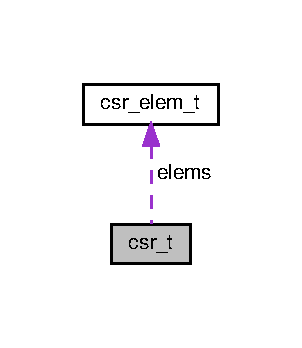
\includegraphics[width=145pt]{structcsr__t__coll__graph}
\end{center}
\end{figure}
\subsection*{Public Attributes}
\begin{DoxyCompactItemize}
\item 
\hyperlink{spmv_8cc_a8e93478a00e685bea5e6a3f617bf03a3}{idx\+\_\+t} $\ast$ \hyperlink{structcsr__t_ac52d7a1ff3a054e2b8c7fcc706e525b6}{row\+\_\+start}
\item 
\hyperlink{structcsr__elem__t}{csr\+\_\+elem\+\_\+t} $\ast$ \hyperlink{structcsr__t_a8fda532ad93e6820aad02feac6bbe04b}{elems}
\end{DoxyCompactItemize}


\subsection{Detailed Description}
sparse matrix in compressed row format 

\subsection{Member Data Documentation}
\mbox{\Hypertarget{structcsr__t_a8fda532ad93e6820aad02feac6bbe04b}\label{structcsr__t_a8fda532ad93e6820aad02feac6bbe04b}} 
\index{csr\+\_\+t@{csr\+\_\+t}!elems@{elems}}
\index{elems@{elems}!csr\+\_\+t@{csr\+\_\+t}}
\subsubsection{\texorpdfstring{elems}{elems}}
{\footnotesize\ttfamily \hyperlink{structcsr__elem__t}{csr\+\_\+elem\+\_\+t}$\ast$ csr\+\_\+t\+::elems}

elements array \mbox{\Hypertarget{structcsr__t_ac52d7a1ff3a054e2b8c7fcc706e525b6}\label{structcsr__t_ac52d7a1ff3a054e2b8c7fcc706e525b6}} 
\index{csr\+\_\+t@{csr\+\_\+t}!row\+\_\+start@{row\+\_\+start}}
\index{row\+\_\+start@{row\+\_\+start}!csr\+\_\+t@{csr\+\_\+t}}
\subsubsection{\texorpdfstring{row\+\_\+start}{row\_start}}
{\footnotesize\ttfamily \hyperlink{spmv_8cc_a8e93478a00e685bea5e6a3f617bf03a3}{idx\+\_\+t}$\ast$ csr\+\_\+t\+::row\+\_\+start}

elems\mbox{[}row\+\_\+start\mbox{[}i\mbox{]}\mbox{]} is the first element of row i 

The documentation for this struct was generated from the following file\+:\begin{DoxyCompactItemize}
\item 
/home/tau/public\+\_\+html/lecture/parallel\+\_\+distributed/2018/parallel-\/distributed-\/handson/03spmv/\hyperlink{spmv_8cc}{spmv.\+cc}\end{DoxyCompactItemize}

\hypertarget{structsparse__t}{}\section{sparse\+\_\+t Struct Reference}
\label{structsparse__t}\index{sparse\+\_\+t@{sparse\+\_\+t}}


sparse matrix (in any format)  




Collaboration diagram for sparse\+\_\+t\+:\nopagebreak
\begin{figure}[H]
\begin{center}
\leavevmode
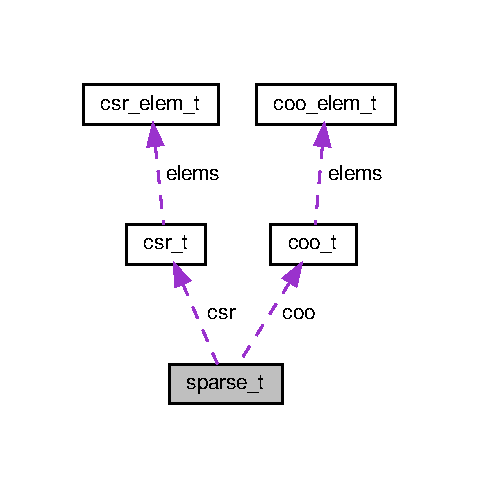
\includegraphics[width=230pt]{structsparse__t__coll__graph}
\end{center}
\end{figure}
\subsection*{Public Attributes}
\begin{DoxyCompactItemize}
\item 
\hyperlink{spmv_8cc_a8c0094893526c01b430903b2d9227256}{sparse\+\_\+format\+\_\+t} \hyperlink{structsparse__t_a1bb9e61c965f9ea814aab21f7ff77a73}{format}
\item 
\hyperlink{spmv_8cc_a8e93478a00e685bea5e6a3f617bf03a3}{idx\+\_\+t} \hyperlink{structsparse__t_a8a08bd7a16c76180afccf05e28f72a93}{M}
\item 
\hyperlink{spmv_8cc_a8e93478a00e685bea5e6a3f617bf03a3}{idx\+\_\+t} \hyperlink{structsparse__t_a418c6deef17a60f31ff11182ea94f85a}{N}
\item 
\hyperlink{spmv_8cc_a8e93478a00e685bea5e6a3f617bf03a3}{idx\+\_\+t} \hyperlink{structsparse__t_ae982d138f3904323b65975769b045a3f}{nnz}
\item 
\mbox{\Hypertarget{structsparse__t_a4d180146ce4a12b0d990cf0e803f7e64}\label{structsparse__t_a4d180146ce4a12b0d990cf0e803f7e64}} 
\begin{tabbing}
xx\=xx\=xx\=xx\=xx\=xx\=xx\=xx\=xx\=\kill
union \{\\
\>\hyperlink{structcoo__t}{coo\_t} \hyperlink{structsparse__t_ad0391f2782f49ea2eb248ed255e9d732}{coo}\\
\>\hyperlink{structcsr__t}{csr\_t} \hyperlink{structsparse__t_a68a71613181b0380d0d4d871236b2521}{csr}\\
\}; \\

\end{tabbing}\end{DoxyCompactItemize}


\subsection{Detailed Description}
sparse matrix (in any format) 

\subsection{Member Data Documentation}
\mbox{\Hypertarget{structsparse__t_ad0391f2782f49ea2eb248ed255e9d732}\label{structsparse__t_ad0391f2782f49ea2eb248ed255e9d732}} 
\index{sparse\+\_\+t@{sparse\+\_\+t}!coo@{coo}}
\index{coo@{coo}!sparse\+\_\+t@{sparse\+\_\+t}}
\subsubsection{\texorpdfstring{coo}{coo}}
{\footnotesize\ttfamily \hyperlink{structcoo__t}{coo\+\_\+t} sparse\+\_\+t\+::coo}

coo or sorted coo \mbox{\Hypertarget{structsparse__t_a68a71613181b0380d0d4d871236b2521}\label{structsparse__t_a68a71613181b0380d0d4d871236b2521}} 
\index{sparse\+\_\+t@{sparse\+\_\+t}!csr@{csr}}
\index{csr@{csr}!sparse\+\_\+t@{sparse\+\_\+t}}
\subsubsection{\texorpdfstring{csr}{csr}}
{\footnotesize\ttfamily \hyperlink{structcsr__t}{csr\+\_\+t} sparse\+\_\+t\+::csr}

csr \mbox{\Hypertarget{structsparse__t_a1bb9e61c965f9ea814aab21f7ff77a73}\label{structsparse__t_a1bb9e61c965f9ea814aab21f7ff77a73}} 
\index{sparse\+\_\+t@{sparse\+\_\+t}!format@{format}}
\index{format@{format}!sparse\+\_\+t@{sparse\+\_\+t}}
\subsubsection{\texorpdfstring{format}{format}}
{\footnotesize\ttfamily \hyperlink{spmv_8cc_a8c0094893526c01b430903b2d9227256}{sparse\+\_\+format\+\_\+t} sparse\+\_\+t\+::format}

format \mbox{\Hypertarget{structsparse__t_a8a08bd7a16c76180afccf05e28f72a93}\label{structsparse__t_a8a08bd7a16c76180afccf05e28f72a93}} 
\index{sparse\+\_\+t@{sparse\+\_\+t}!M@{M}}
\index{M@{M}!sparse\+\_\+t@{sparse\+\_\+t}}
\subsubsection{\texorpdfstring{M}{M}}
{\footnotesize\ttfamily \hyperlink{spmv_8cc_a8e93478a00e685bea5e6a3f617bf03a3}{idx\+\_\+t} sparse\+\_\+t\+::M}

number of rows \mbox{\Hypertarget{structsparse__t_a418c6deef17a60f31ff11182ea94f85a}\label{structsparse__t_a418c6deef17a60f31ff11182ea94f85a}} 
\index{sparse\+\_\+t@{sparse\+\_\+t}!N@{N}}
\index{N@{N}!sparse\+\_\+t@{sparse\+\_\+t}}
\subsubsection{\texorpdfstring{N}{N}}
{\footnotesize\ttfamily \hyperlink{spmv_8cc_a8e93478a00e685bea5e6a3f617bf03a3}{idx\+\_\+t} sparse\+\_\+t\+::N}

number of columns \mbox{\Hypertarget{structsparse__t_ae982d138f3904323b65975769b045a3f}\label{structsparse__t_ae982d138f3904323b65975769b045a3f}} 
\index{sparse\+\_\+t@{sparse\+\_\+t}!nnz@{nnz}}
\index{nnz@{nnz}!sparse\+\_\+t@{sparse\+\_\+t}}
\subsubsection{\texorpdfstring{nnz}{nnz}}
{\footnotesize\ttfamily \hyperlink{spmv_8cc_a8e93478a00e685bea5e6a3f617bf03a3}{idx\+\_\+t} sparse\+\_\+t\+::nnz}

number of non-\/zeros 

The documentation for this struct was generated from the following file\+:\begin{DoxyCompactItemize}
\item 
/home/tau/public\+\_\+html/lecture/parallel\+\_\+distributed/2018/parallel-\/distributed-\/handson/03spmv/\hyperlink{spmv_8cc}{spmv.\+cc}\end{DoxyCompactItemize}

\hypertarget{structvec__t}{}\section{vec\+\_\+t Struct Reference}
\label{structvec__t}\index{vec\+\_\+t@{vec\+\_\+t}}


vector  


\subsection*{Public Attributes}
\begin{DoxyCompactItemize}
\item 
\hyperlink{spmv_8cc_a8e93478a00e685bea5e6a3f617bf03a3}{idx\+\_\+t} \hyperlink{structvec__t_a06879ff4054298fbc680b02e3e18da7a}{n}
\item 
\hyperlink{spmv_8cc_a11d147c64891830c9e79b3315b1b2e21}{real} $\ast$ \hyperlink{structvec__t_af9bc087be96662c10187c01cf9bfc834}{elems}
\end{DoxyCompactItemize}


\subsection{Detailed Description}
vector 

\subsection{Member Data Documentation}
\mbox{\Hypertarget{structvec__t_af9bc087be96662c10187c01cf9bfc834}\label{structvec__t_af9bc087be96662c10187c01cf9bfc834}} 
\index{vec\+\_\+t@{vec\+\_\+t}!elems@{elems}}
\index{elems@{elems}!vec\+\_\+t@{vec\+\_\+t}}
\subsubsection{\texorpdfstring{elems}{elems}}
{\footnotesize\ttfamily \hyperlink{spmv_8cc_a11d147c64891830c9e79b3315b1b2e21}{real} $\ast$ vec\+\_\+t\+::elems}

array of elements \mbox{\Hypertarget{structvec__t_a06879ff4054298fbc680b02e3e18da7a}\label{structvec__t_a06879ff4054298fbc680b02e3e18da7a}} 
\index{vec\+\_\+t@{vec\+\_\+t}!n@{n}}
\index{n@{n}!vec\+\_\+t@{vec\+\_\+t}}
\subsubsection{\texorpdfstring{n}{n}}
{\footnotesize\ttfamily \hyperlink{spmv_8cc_a8e93478a00e685bea5e6a3f617bf03a3}{idx\+\_\+t} vec\+\_\+t\+::n}

number of elements 

The documentation for this struct was generated from the following files\+:\begin{DoxyCompactItemize}
\item 
/home/tau/public\+\_\+html/lecture/parallel\+\_\+distributed/2018/parallel-\/distributed-\/handson/03spmv/\hyperlink{spmv_8cc}{spmv.\+cc}\item 
/home/tau/public\+\_\+html/lecture/parallel\+\_\+distributed/2018/parallel-\/distributed-\/handson/03spmv/spmvx.\+cc\end{DoxyCompactItemize}

\chapter{File Documentation}
\hypertarget{spmv_8cc}{}\section{/home/tau/public\+\_\+html/lecture/parallel\+\_\+distributed/2018/ex/00spmv/spmv.cc File Reference}
\label{spmv_8cc}\index{/home/tau/public\+\_\+html/lecture/parallel\+\_\+distributed/2018/ex/00spmv/spmv.\+cc@{/home/tau/public\+\_\+html/lecture/parallel\+\_\+distributed/2018/ex/00spmv/spmv.\+cc}}


sparse matrix vector multiplication  


{\ttfamily \#include $<$assert.\+h$>$}\newline
{\ttfamily \#include $<$math.\+h$>$}\newline
{\ttfamily \#include $<$stdio.\+h$>$}\newline
{\ttfamily \#include $<$stdlib.\+h$>$}\newline
{\ttfamily \#include $<$string.\+h$>$}\newline
{\ttfamily \#include $<$getopt.\+h$>$}\newline
{\ttfamily \#include $<$time.\+h$>$}\newline
Include dependency graph for spmv.\+cc\+:
\nopagebreak
\begin{figure}[H]
\begin{center}
\leavevmode
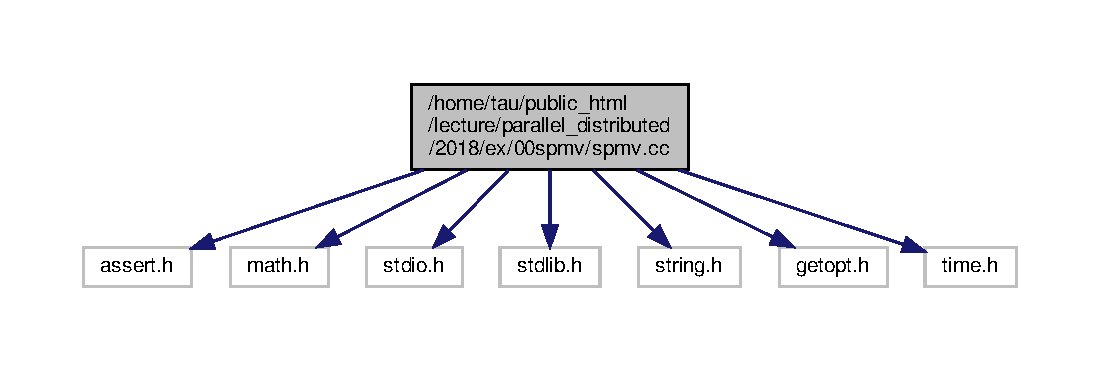
\includegraphics[width=350pt]{spmv_8cc__incl}
\end{center}
\end{figure}
\subsection*{Classes}
\begin{DoxyCompactItemize}
\item 
struct \hyperlink{structcoo__elem__t}{coo\+\_\+elem\+\_\+t}
\begin{DoxyCompactList}\small\item\em an element of coordinate list (i, j, a) \end{DoxyCompactList}\item 
struct \hyperlink{structcsr__elem__t}{csr\+\_\+elem\+\_\+t}
\begin{DoxyCompactList}\small\item\em an element of compressed sparse row \end{DoxyCompactList}\item 
struct \hyperlink{structcoo__t}{coo\+\_\+t}
\begin{DoxyCompactList}\small\item\em sparse matrix in coodinate list format \end{DoxyCompactList}\item 
struct \hyperlink{structcsr__t}{csr\+\_\+t}
\begin{DoxyCompactList}\small\item\em sparse matrix in compressed row format \end{DoxyCompactList}\item 
struct \hyperlink{structsparse__t}{sparse\+\_\+t}
\begin{DoxyCompactList}\small\item\em sparse matrix (in any format) \end{DoxyCompactList}\item 
struct \hyperlink{structvec__t}{vec\+\_\+t}
\begin{DoxyCompactList}\small\item\em vector \end{DoxyCompactList}\item 
struct \hyperlink{structcmdline__options__t}{cmdline\+\_\+options\+\_\+t}
\begin{DoxyCompactList}\small\item\em command line option \end{DoxyCompactList}\end{DoxyCompactItemize}
\subsection*{Typedefs}
\begin{DoxyCompactItemize}
\item 
\mbox{\Hypertarget{spmv_8cc_a8e93478a00e685bea5e6a3f617bf03a3}\label{spmv_8cc_a8e93478a00e685bea5e6a3f617bf03a3}} 
typedef int \hyperlink{spmv_8cc_a8e93478a00e685bea5e6a3f617bf03a3}{idx\+\_\+t}
\begin{DoxyCompactList}\small\item\em type of matrix index (i,j,...) \end{DoxyCompactList}\item 
\mbox{\Hypertarget{spmv_8cc_a11d147c64891830c9e79b3315b1b2e21}\label{spmv_8cc_a11d147c64891830c9e79b3315b1b2e21}} 
typedef double \hyperlink{spmv_8cc_a11d147c64891830c9e79b3315b1b2e21}{real}
\begin{DoxyCompactList}\small\item\em type of a matrix element \end{DoxyCompactList}\end{DoxyCompactItemize}
\subsection*{Enumerations}
\begin{DoxyCompactItemize}
\item 
enum \hyperlink{spmv_8cc_a8c0094893526c01b430903b2d9227256}{sparse\+\_\+format\+\_\+t} \{ \hyperlink{spmv_8cc_a8c0094893526c01b430903b2d9227256a3873dfc9b4303f69130d325bb9d5d3d9}{sparse\+\_\+format\+\_\+coo}, 
\hyperlink{spmv_8cc_a8c0094893526c01b430903b2d9227256ae622b3c6575c5efae6930339af50e076}{sparse\+\_\+format\+\_\+coo\+\_\+sorted}, 
\hyperlink{spmv_8cc_a8c0094893526c01b430903b2d9227256a8d3a61cb0ac76c8b5334c24c7618c4c7}{sparse\+\_\+format\+\_\+csr}, 
\hyperlink{spmv_8cc_a8c0094893526c01b430903b2d9227256adc326179d0d559f82edc8cd35be11de5}{sparse\+\_\+format\+\_\+invalid}
 \}\begin{DoxyCompactList}\small\item\em sparse matrix storage format \end{DoxyCompactList}
\item 
enum \hyperlink{spmv_8cc_ad2cf0493af54bf76c5be68b4634fcab7}{spmv\+\_\+algo\+\_\+t} \{ \hyperlink{spmv_8cc_ad2cf0493af54bf76c5be68b4634fcab7a8239a128e5970e7f36aec71d6265d78a}{spmv\+\_\+algo\+\_\+serial}, 
\hyperlink{spmv_8cc_ad2cf0493af54bf76c5be68b4634fcab7abbdcd58ce962bc8134af08a7f4310f81}{spmv\+\_\+algo\+\_\+parallel}, 
{\bfseries spmv\+\_\+algo\+\_\+invalid}
 \}\begin{DoxyCompactList}\small\item\em spmv matrix algorithm \end{DoxyCompactList}
\end{DoxyCompactItemize}
\subsection*{Functions}
\begin{DoxyCompactItemize}
\item 
\mbox{\Hypertarget{spmv_8cc_a79a33f2f3ea6bfd4bd5fc8bc1c026a5b}\label{spmv_8cc_a79a33f2f3ea6bfd4bd5fc8bc1c026a5b}} 
void $\ast$ \hyperlink{spmv_8cc_a79a33f2f3ea6bfd4bd5fc8bc1c026a5b}{xalloc} (size\+\_\+t sz)
\begin{DoxyCompactList}\small\item\em malloc + check \end{DoxyCompactList}\item 
\mbox{\Hypertarget{spmv_8cc_a3ef938bd87c574f4deb4e5b05de27fc2}\label{spmv_8cc_a3ef938bd87c574f4deb4e5b05de27fc2}} 
void \hyperlink{spmv_8cc_a3ef938bd87c574f4deb4e5b05de27fc2}{xfree} (void $\ast$a)
\begin{DoxyCompactList}\small\item\em wrap free \end{DoxyCompactList}\item 
\mbox{\Hypertarget{spmv_8cc_a886d462f047a9680c3a5b9359a082469}\label{spmv_8cc_a886d462f047a9680c3a5b9359a082469}} 
void \hyperlink{spmv_8cc_a886d462f047a9680c3a5b9359a082469}{coo\+\_\+destroy} (\hyperlink{structsparse__t}{sparse\+\_\+t} A)
\begin{DoxyCompactList}\small\item\em destroy coo \end{DoxyCompactList}\item 
\mbox{\Hypertarget{spmv_8cc_a3ae3b530bd4c6af7148b8d6f0350d5b7}\label{spmv_8cc_a3ae3b530bd4c6af7148b8d6f0350d5b7}} 
void \hyperlink{spmv_8cc_a3ae3b530bd4c6af7148b8d6f0350d5b7}{csr\+\_\+destroy} (\hyperlink{structsparse__t}{sparse\+\_\+t} A)
\begin{DoxyCompactList}\small\item\em destroy csr \end{DoxyCompactList}\item 
\mbox{\Hypertarget{spmv_8cc_a9743d89de22a2978402684c73921c2f7}\label{spmv_8cc_a9743d89de22a2978402684c73921c2f7}} 
void \hyperlink{spmv_8cc_a9743d89de22a2978402684c73921c2f7}{sparse\+\_\+destroy} (\hyperlink{structsparse__t}{sparse\+\_\+t} A)
\begin{DoxyCompactList}\small\item\em destroy sparse matrix in any format \end{DoxyCompactList}\item 
\mbox{\Hypertarget{spmv_8cc_a174b34f4428f02a25bcaf8bb40309198}\label{spmv_8cc_a174b34f4428f02a25bcaf8bb40309198}} 
void \hyperlink{spmv_8cc_a174b34f4428f02a25bcaf8bb40309198}{vec\+\_\+destroy} (\hyperlink{structvec__t}{vec\+\_\+t} x)
\begin{DoxyCompactList}\small\item\em destroy vector \end{DoxyCompactList}\item 
\mbox{\Hypertarget{spmv_8cc_ab4eb7b1ede09476134c12ed6a60687b5}\label{spmv_8cc_ab4eb7b1ede09476134c12ed6a60687b5}} 
\hyperlink{structsparse__t}{sparse\+\_\+t} \hyperlink{spmv_8cc_ab4eb7b1ede09476134c12ed6a60687b5}{mk\+\_\+coo\+\_\+random} (\hyperlink{spmv_8cc_a8e93478a00e685bea5e6a3f617bf03a3}{idx\+\_\+t} M, \hyperlink{spmv_8cc_a8e93478a00e685bea5e6a3f617bf03a3}{idx\+\_\+t} N, \hyperlink{spmv_8cc_a8e93478a00e685bea5e6a3f617bf03a3}{idx\+\_\+t} nnz, unsigned short rg\mbox{[}3\mbox{]})
\begin{DoxyCompactList}\small\item\em make a random coo matrix \end{DoxyCompactList}\item 
\mbox{\Hypertarget{spmv_8cc_a2429d70711dfd86b1a7ed6f5b72be673}\label{spmv_8cc_a2429d70711dfd86b1a7ed6f5b72be673}} 
int \hyperlink{spmv_8cc_a2429d70711dfd86b1a7ed6f5b72be673}{coo\+\_\+elem\+\_\+cmp} (const void $\ast$a\+\_\+, const void $\ast$b\+\_\+)
\begin{DoxyCompactList}\small\item\em compare two coo elements \end{DoxyCompactList}\item 
\mbox{\Hypertarget{spmv_8cc_ae3c168861ef8e87bf6189ae4d2e24883}\label{spmv_8cc_ae3c168861ef8e87bf6189ae4d2e24883}} 
\hyperlink{structsparse__t}{sparse\+\_\+t} \hyperlink{spmv_8cc_ae3c168861ef8e87bf6189ae4d2e24883}{coo\+\_\+to\+\_\+coo\+\_\+sorted} (\hyperlink{structsparse__t}{sparse\+\_\+t} A, int in\+\_\+place)
\begin{DoxyCompactList}\small\item\em convert A to coo\+\_\+sorted format. if in\+\_\+place is true, update elements of A in place. \end{DoxyCompactList}\item 
\mbox{\Hypertarget{spmv_8cc_a54b858a5780a6aa5027b9dae5fb7906b}\label{spmv_8cc_a54b858a5780a6aa5027b9dae5fb7906b}} 
\hyperlink{structsparse__t}{sparse\+\_\+t} \hyperlink{spmv_8cc_a54b858a5780a6aa5027b9dae5fb7906b}{mk\+\_\+coo\+\_\+sorted\+\_\+random} (\hyperlink{spmv_8cc_a8e93478a00e685bea5e6a3f617bf03a3}{idx\+\_\+t} M, \hyperlink{spmv_8cc_a8e93478a00e685bea5e6a3f617bf03a3}{idx\+\_\+t} N, \hyperlink{spmv_8cc_a8e93478a00e685bea5e6a3f617bf03a3}{idx\+\_\+t} nnz, unsigned short rg\mbox{[}3\mbox{]})
\begin{DoxyCompactList}\small\item\em make a random coo matrix, with elements sorted in the dictionary order of (i, j) \end{DoxyCompactList}\item 
\hyperlink{structsparse__t}{sparse\+\_\+t} \hyperlink{spmv_8cc_a92703aefc64c5c8929dc483a0434c637}{coo\+\_\+to\+\_\+csr} (\hyperlink{structsparse__t}{sparse\+\_\+t} A, int update\+\_\+A)
\begin{DoxyCompactList}\small\item\em coo -\/$>$ csr \end{DoxyCompactList}\item 
\mbox{\Hypertarget{spmv_8cc_af13023640a314474736dfc03be80b500}\label{spmv_8cc_af13023640a314474736dfc03be80b500}} 
\hyperlink{structsparse__t}{sparse\+\_\+t} \hyperlink{spmv_8cc_af13023640a314474736dfc03be80b500}{csr\+\_\+to\+\_\+coo} (\hyperlink{structsparse__t}{sparse\+\_\+t} A)
\begin{DoxyCompactList}\small\item\em csr -\/$>$ coo \end{DoxyCompactList}\item 
\mbox{\Hypertarget{spmv_8cc_ab5e761ffaea4d448caa367585792f23c}\label{spmv_8cc_ab5e761ffaea4d448caa367585792f23c}} 
\hyperlink{structsparse__t}{sparse\+\_\+t} \hyperlink{spmv_8cc_ab5e761ffaea4d448caa367585792f23c}{mk\+\_\+csr\+\_\+random} (\hyperlink{spmv_8cc_a8e93478a00e685bea5e6a3f617bf03a3}{idx\+\_\+t} M, \hyperlink{spmv_8cc_a8e93478a00e685bea5e6a3f617bf03a3}{idx\+\_\+t} N, \hyperlink{spmv_8cc_a8e93478a00e685bea5e6a3f617bf03a3}{idx\+\_\+t} nnz, unsigned short rg\mbox{[}3\mbox{]})
\begin{DoxyCompactList}\small\item\em make a random csr matrix \end{DoxyCompactList}\item 
\mbox{\Hypertarget{spmv_8cc_a9936542a2f858311996f17bdf8996264}\label{spmv_8cc_a9936542a2f858311996f17bdf8996264}} 
\hyperlink{structsparse__t}{sparse\+\_\+t} \hyperlink{spmv_8cc_a9936542a2f858311996f17bdf8996264}{mk\+\_\+sparse\+\_\+random} (\hyperlink{spmv_8cc_a8c0094893526c01b430903b2d9227256}{sparse\+\_\+format\+\_\+t} format, \hyperlink{spmv_8cc_a8e93478a00e685bea5e6a3f617bf03a3}{idx\+\_\+t} M, \hyperlink{spmv_8cc_a8e93478a00e685bea5e6a3f617bf03a3}{idx\+\_\+t} N, \hyperlink{spmv_8cc_a8e93478a00e685bea5e6a3f617bf03a3}{idx\+\_\+t} nnz, unsigned short rg\mbox{[}3\mbox{]})
\begin{DoxyCompactList}\small\item\em make a random sparse matrix of kind (coo, csr, etc.) \end{DoxyCompactList}\item 
\mbox{\Hypertarget{spmv_8cc_aef0dc6d491152684cdeba40fa8a98010}\label{spmv_8cc_aef0dc6d491152684cdeba40fa8a98010}} 
\hyperlink{structsparse__t}{sparse\+\_\+t} \hyperlink{spmv_8cc_aef0dc6d491152684cdeba40fa8a98010}{coo\+\_\+transpose} (\hyperlink{structsparse__t}{sparse\+\_\+t} A, int in\+\_\+place)
\begin{DoxyCompactList}\small\item\em transpose a matrix in coordinate list format \end{DoxyCompactList}\item 
\mbox{\Hypertarget{spmv_8cc_ad530dc3dbde6b6ee8e075bb82e38a0a5}\label{spmv_8cc_ad530dc3dbde6b6ee8e075bb82e38a0a5}} 
\hyperlink{structsparse__t}{sparse\+\_\+t} \hyperlink{spmv_8cc_ad530dc3dbde6b6ee8e075bb82e38a0a5}{sparse\+\_\+transpose} (\hyperlink{structsparse__t}{sparse\+\_\+t} A)
\begin{DoxyCompactList}\small\item\em transpose a matrix in any format \end{DoxyCompactList}\item 
\mbox{\Hypertarget{spmv_8cc_a8a1ce86dfa6920a65796860f1b7fd858}\label{spmv_8cc_a8a1ce86dfa6920a65796860f1b7fd858}} 
long \hyperlink{spmv_8cc_a8a1ce86dfa6920a65796860f1b7fd858}{spmv\+\_\+coo\+\_\+serial} (\hyperlink{structsparse__t}{sparse\+\_\+t} A, \hyperlink{structvec__t}{vec\+\_\+t} vx, \hyperlink{structvec__t}{vec\+\_\+t} vy)
\begin{DoxyCompactList}\small\item\em y = A $\ast$ x in serial for coordinate list format \end{DoxyCompactList}\item 
\mbox{\Hypertarget{spmv_8cc_ab5f800ac71c8b2ffded8bb69e4f584fe}\label{spmv_8cc_ab5f800ac71c8b2ffded8bb69e4f584fe}} 
long \hyperlink{spmv_8cc_ab5f800ac71c8b2ffded8bb69e4f584fe}{spmv\+\_\+coo\+\_\+parallel} (\hyperlink{structsparse__t}{sparse\+\_\+t} A, \hyperlink{structvec__t}{vec\+\_\+t} vx, \hyperlink{structvec__t}{vec\+\_\+t} vy)
\begin{DoxyCompactList}\small\item\em y = A $\ast$ x in parallel for coordinate list format \end{DoxyCompactList}\item 
\mbox{\Hypertarget{spmv_8cc_a2c2f88615681aac89eb9a972b2ef24c3}\label{spmv_8cc_a2c2f88615681aac89eb9a972b2ef24c3}} 
long \hyperlink{spmv_8cc_a2c2f88615681aac89eb9a972b2ef24c3}{spmv\+\_\+coo} (\hyperlink{spmv_8cc_ad2cf0493af54bf76c5be68b4634fcab7}{spmv\+\_\+algo\+\_\+t} algo, \hyperlink{structsparse__t}{sparse\+\_\+t} A, \hyperlink{structvec__t}{vec\+\_\+t} x, \hyperlink{structvec__t}{vec\+\_\+t} y)
\begin{DoxyCompactList}\small\item\em y = A $\ast$ x for coordinate list format \end{DoxyCompactList}\item 
\mbox{\Hypertarget{spmv_8cc_ac028553adb9a6c59a82109179f5e8d51}\label{spmv_8cc_ac028553adb9a6c59a82109179f5e8d51}} 
long \hyperlink{spmv_8cc_ac028553adb9a6c59a82109179f5e8d51}{spmv\+\_\+csr\+\_\+serial} (\hyperlink{structsparse__t}{sparse\+\_\+t} A, \hyperlink{structvec__t}{vec\+\_\+t} vx, \hyperlink{structvec__t}{vec\+\_\+t} vy)
\begin{DoxyCompactList}\small\item\em y = A $\ast$ x in serial for csr format \end{DoxyCompactList}\item 
\mbox{\Hypertarget{spmv_8cc_a0a599d46a47b7019b7083f2aa3847ac1}\label{spmv_8cc_a0a599d46a47b7019b7083f2aa3847ac1}} 
long \hyperlink{spmv_8cc_a0a599d46a47b7019b7083f2aa3847ac1}{spmv\+\_\+csr\+\_\+parallel} (\hyperlink{structsparse__t}{sparse\+\_\+t} A, \hyperlink{structvec__t}{vec\+\_\+t} vx, \hyperlink{structvec__t}{vec\+\_\+t} vy)
\begin{DoxyCompactList}\small\item\em y = A $\ast$ x in parallel for csr format \end{DoxyCompactList}\item 
\mbox{\Hypertarget{spmv_8cc_a2a769e363b1cf135e05e68c57e070eba}\label{spmv_8cc_a2a769e363b1cf135e05e68c57e070eba}} 
long \hyperlink{spmv_8cc_a2a769e363b1cf135e05e68c57e070eba}{spmv\+\_\+csr} (\hyperlink{spmv_8cc_ad2cf0493af54bf76c5be68b4634fcab7}{spmv\+\_\+algo\+\_\+t} algo, \hyperlink{structsparse__t}{sparse\+\_\+t} A, \hyperlink{structvec__t}{vec\+\_\+t} x, \hyperlink{structvec__t}{vec\+\_\+t} y)
\begin{DoxyCompactList}\small\item\em y = A $\ast$ x for csr format \end{DoxyCompactList}\item 
\mbox{\Hypertarget{spmv_8cc_ad8db62e7d883972f292708fd2d963714}\label{spmv_8cc_ad8db62e7d883972f292708fd2d963714}} 
long \hyperlink{spmv_8cc_ad8db62e7d883972f292708fd2d963714}{spmv} (\hyperlink{spmv_8cc_ad2cf0493af54bf76c5be68b4634fcab7}{spmv\+\_\+algo\+\_\+t} algo, \hyperlink{structsparse__t}{sparse\+\_\+t} A, \hyperlink{structvec__t}{vec\+\_\+t} x, \hyperlink{structvec__t}{vec\+\_\+t} y)
\begin{DoxyCompactList}\small\item\em y = A $\ast$ x \end{DoxyCompactList}\item 
\mbox{\Hypertarget{spmv_8cc_a3f92724879c2d612bf5310ab707724cd}\label{spmv_8cc_a3f92724879c2d612bf5310ab707724cd}} 
\hyperlink{spmv_8cc_a11d147c64891830c9e79b3315b1b2e21}{real} \hyperlink{spmv_8cc_a3f92724879c2d612bf5310ab707724cd}{vec\+\_\+norm2} (\hyperlink{structvec__t}{vec\+\_\+t} v)
\begin{DoxyCompactList}\small\item\em square norm of a vector \end{DoxyCompactList}\item 
\mbox{\Hypertarget{spmv_8cc_a131c8ac0a310b45de83d8ba4aee5daa2}\label{spmv_8cc_a131c8ac0a310b45de83d8ba4aee5daa2}} 
\hyperlink{spmv_8cc_a11d147c64891830c9e79b3315b1b2e21}{real} \hyperlink{spmv_8cc_a131c8ac0a310b45de83d8ba4aee5daa2}{vec\+\_\+normalize} (\hyperlink{structvec__t}{vec\+\_\+t} v)
\begin{DoxyCompactList}\small\item\em normalize a vector \end{DoxyCompactList}\item 
\mbox{\Hypertarget{spmv_8cc_a1cf75d2ce89a2cc6dd553506b6ac7fae}\label{spmv_8cc_a1cf75d2ce89a2cc6dd553506b6ac7fae}} 
long \hyperlink{spmv_8cc_a1cf75d2ce89a2cc6dd553506b6ac7fae}{cur\+\_\+time\+\_\+ns} ()
\begin{DoxyCompactList}\small\item\em current time in nano second \end{DoxyCompactList}\item 
\mbox{\Hypertarget{spmv_8cc_aec765aa23a1aa4d745c881c2c35622cf}\label{spmv_8cc_aec765aa23a1aa4d745c881c2c35622cf}} 
\hyperlink{spmv_8cc_a11d147c64891830c9e79b3315b1b2e21}{real} \hyperlink{spmv_8cc_aec765aa23a1aa4d745c881c2c35622cf}{repeat\+\_\+spmv} (\hyperlink{spmv_8cc_ad2cf0493af54bf76c5be68b4634fcab7}{spmv\+\_\+algo\+\_\+t} algo, \hyperlink{structsparse__t}{sparse\+\_\+t} A, \hyperlink{structsparse__t}{sparse\+\_\+t} tA, \hyperlink{structvec__t}{vec\+\_\+t} x, \hyperlink{structvec__t}{vec\+\_\+t} y, \hyperlink{spmv_8cc_a8e93478a00e685bea5e6a3f617bf03a3}{idx\+\_\+t} repeat)
\begin{DoxyCompactList}\small\item\em repeat y = A x; x = tA y; many times \end{DoxyCompactList}\item 
\mbox{\Hypertarget{spmv_8cc_ad7949349d6b359f1fe6350b4d46fadb8}\label{spmv_8cc_ad7949349d6b359f1fe6350b4d46fadb8}} 
\hyperlink{structvec__t}{vec\+\_\+t} \hyperlink{spmv_8cc_ad7949349d6b359f1fe6350b4d46fadb8}{mk\+\_\+vec\+\_\+random} (\hyperlink{spmv_8cc_a8e93478a00e685bea5e6a3f617bf03a3}{idx\+\_\+t} n, unsigned short rg\mbox{[}3\mbox{]})
\begin{DoxyCompactList}\small\item\em make a random vector \end{DoxyCompactList}\item 
\mbox{\Hypertarget{spmv_8cc_a7087e5f081d6e211cbca607dc03aedfa}\label{spmv_8cc_a7087e5f081d6e211cbca607dc03aedfa}} 
\hyperlink{structvec__t}{vec\+\_\+t} \hyperlink{spmv_8cc_a7087e5f081d6e211cbca607dc03aedfa}{mk\+\_\+vec\+\_\+unit\+\_\+random} (\hyperlink{spmv_8cc_a8e93478a00e685bea5e6a3f617bf03a3}{idx\+\_\+t} n, unsigned short rg\mbox{[}3\mbox{]})
\begin{DoxyCompactList}\small\item\em make a unit-\/length random vector \end{DoxyCompactList}\item 
\mbox{\Hypertarget{spmv_8cc_a22ac9fee564d3ed893e7a57af08d65b9}\label{spmv_8cc_a22ac9fee564d3ed893e7a57af08d65b9}} 
\hyperlink{structvec__t}{vec\+\_\+t} \hyperlink{spmv_8cc_a22ac9fee564d3ed893e7a57af08d65b9}{mk\+\_\+vec\+\_\+zero} (\hyperlink{spmv_8cc_a8e93478a00e685bea5e6a3f617bf03a3}{idx\+\_\+t} n)
\begin{DoxyCompactList}\small\item\em make a zero vector \end{DoxyCompactList}\item 
\mbox{\Hypertarget{spmv_8cc_a09b8e85d2892697f77b3b0eeae5de59a}\label{spmv_8cc_a09b8e85d2892697f77b3b0eeae5de59a}} 
\hyperlink{structcmdline__options__t}{cmdline\+\_\+options\+\_\+t} \hyperlink{spmv_8cc_a09b8e85d2892697f77b3b0eeae5de59a}{default\+\_\+opts} ()
\begin{DoxyCompactList}\small\item\em default values for command line options \end{DoxyCompactList}\item 
\mbox{\Hypertarget{spmv_8cc_a10ca6251cec6f3b812ec1a3ee9a81501}\label{spmv_8cc_a10ca6251cec6f3b812ec1a3ee9a81501}} 
\hyperlink{spmv_8cc_a8c0094893526c01b430903b2d9227256}{sparse\+\_\+format\+\_\+t} \hyperlink{spmv_8cc_a10ca6251cec6f3b812ec1a3ee9a81501}{parse\+\_\+sparse\+\_\+format} (char $\ast$s)
\begin{DoxyCompactList}\small\item\em parse a string for matrix format and return an enum value \end{DoxyCompactList}\item 
\mbox{\Hypertarget{spmv_8cc_aefe1c65fa2eb16b63ce6663af0f07af6}\label{spmv_8cc_aefe1c65fa2eb16b63ce6663af0f07af6}} 
\hyperlink{spmv_8cc_ad2cf0493af54bf76c5be68b4634fcab7}{spmv\+\_\+algo\+\_\+t} \hyperlink{spmv_8cc_aefe1c65fa2eb16b63ce6663af0f07af6}{parse\+\_\+spmv\+\_\+algo} (char $\ast$s)
\begin{DoxyCompactList}\small\item\em parse a string for spmv algo and return an enum value \end{DoxyCompactList}\item 
\mbox{\Hypertarget{spmv_8cc_a9da0c69919e3b08e9df0bf1affb54804}\label{spmv_8cc_a9da0c69919e3b08e9df0bf1affb54804}} 
void \hyperlink{spmv_8cc_a9da0c69919e3b08e9df0bf1affb54804}{cmdline\+\_\+options\+\_\+destroy} (\hyperlink{structcmdline__options__t}{cmdline\+\_\+options\+\_\+t} opt)
\begin{DoxyCompactList}\small\item\em release memory for cmdline\+\_\+options \end{DoxyCompactList}\item 
\mbox{\Hypertarget{spmv_8cc_a364112f4dc61f0649eec6b78e586509d}\label{spmv_8cc_a364112f4dc61f0649eec6b78e586509d}} 
void \hyperlink{spmv_8cc_a364112f4dc61f0649eec6b78e586509d}{usage} (const char $\ast$prog)
\begin{DoxyCompactList}\small\item\em usage \end{DoxyCompactList}\item 
\mbox{\Hypertarget{spmv_8cc_ae46c60a3daf9f5acbb90a2d9c412c550}\label{spmv_8cc_ae46c60a3daf9f5acbb90a2d9c412c550}} 
\hyperlink{structcmdline__options__t}{cmdline\+\_\+options\+\_\+t} \hyperlink{spmv_8cc_ae46c60a3daf9f5acbb90a2d9c412c550}{parse\+\_\+args} (int argc, char $\ast$$\ast$argv)
\begin{DoxyCompactList}\small\item\em parse command line args \end{DoxyCompactList}\item 
\mbox{\Hypertarget{spmv_8cc_a3c04138a5bfe5d72780bb7e82a18e627}\label{spmv_8cc_a3c04138a5bfe5d72780bb7e82a18e627}} 
int \hyperlink{spmv_8cc_a3c04138a5bfe5d72780bb7e82a18e627}{main} (int argc, char $\ast$$\ast$argv)
\begin{DoxyCompactList}\small\item\em main \end{DoxyCompactList}\end{DoxyCompactItemize}
\subsection*{Variables}
\begin{DoxyCompactItemize}
\item 
struct option \hyperlink{spmv_8cc_ab5b68aa8f898c499ca2c3092ecd9e552}{long\+\_\+options} \mbox{[}$\,$\mbox{]}
\begin{DoxyCompactList}\small\item\em command line options \end{DoxyCompactList}\end{DoxyCompactItemize}


\subsection{Detailed Description}
sparse matrix vector multiplication 

\begin{DoxyAuthor}{Author}
Kenjiro Taura 
\end{DoxyAuthor}
\begin{DoxyDate}{Date}
Oct. 14, 2018 
\end{DoxyDate}


\subsection{Enumeration Type Documentation}
\mbox{\Hypertarget{spmv_8cc_a8c0094893526c01b430903b2d9227256}\label{spmv_8cc_a8c0094893526c01b430903b2d9227256}} 
\index{spmv.\+cc@{spmv.\+cc}!sparse\+\_\+format\+\_\+t@{sparse\+\_\+format\+\_\+t}}
\index{sparse\+\_\+format\+\_\+t@{sparse\+\_\+format\+\_\+t}!spmv.\+cc@{spmv.\+cc}}
\subsubsection{\texorpdfstring{sparse\+\_\+format\+\_\+t}{sparse\_format\_t}}
{\footnotesize\ttfamily enum \hyperlink{spmv_8cc_a8c0094893526c01b430903b2d9227256}{sparse\+\_\+format\+\_\+t}}



sparse matrix storage format 

\begin{DoxyEnumFields}{Enumerator}
\raisebox{\heightof{T}}[0pt][0pt]{\index{sparse\+\_\+format\+\_\+coo@{sparse\+\_\+format\+\_\+coo}!spmv.\+cc@{spmv.\+cc}}\index{spmv.\+cc@{spmv.\+cc}!sparse\+\_\+format\+\_\+coo@{sparse\+\_\+format\+\_\+coo}}}\mbox{\Hypertarget{spmv_8cc_a8c0094893526c01b430903b2d9227256a3873dfc9b4303f69130d325bb9d5d3d9}\label{spmv_8cc_a8c0094893526c01b430903b2d9227256a3873dfc9b4303f69130d325bb9d5d3d9}} 
sparse\+\_\+format\+\_\+coo&coordinate list \\
\hline

\raisebox{\heightof{T}}[0pt][0pt]{\index{sparse\+\_\+format\+\_\+coo\+\_\+sorted@{sparse\+\_\+format\+\_\+coo\+\_\+sorted}!spmv.\+cc@{spmv.\+cc}}\index{spmv.\+cc@{spmv.\+cc}!sparse\+\_\+format\+\_\+coo\+\_\+sorted@{sparse\+\_\+format\+\_\+coo\+\_\+sorted}}}\mbox{\Hypertarget{spmv_8cc_a8c0094893526c01b430903b2d9227256ae622b3c6575c5efae6930339af50e076}\label{spmv_8cc_a8c0094893526c01b430903b2d9227256ae622b3c6575c5efae6930339af50e076}} 
sparse\+\_\+format\+\_\+coo\+\_\+sorted&sorted coordinate list \\
\hline

\raisebox{\heightof{T}}[0pt][0pt]{\index{sparse\+\_\+format\+\_\+csr@{sparse\+\_\+format\+\_\+csr}!spmv.\+cc@{spmv.\+cc}}\index{spmv.\+cc@{spmv.\+cc}!sparse\+\_\+format\+\_\+csr@{sparse\+\_\+format\+\_\+csr}}}\mbox{\Hypertarget{spmv_8cc_a8c0094893526c01b430903b2d9227256a8d3a61cb0ac76c8b5334c24c7618c4c7}\label{spmv_8cc_a8c0094893526c01b430903b2d9227256a8d3a61cb0ac76c8b5334c24c7618c4c7}} 
sparse\+\_\+format\+\_\+csr&compressed sparse row \\
\hline

\raisebox{\heightof{T}}[0pt][0pt]{\index{sparse\+\_\+format\+\_\+invalid@{sparse\+\_\+format\+\_\+invalid}!spmv.\+cc@{spmv.\+cc}}\index{spmv.\+cc@{spmv.\+cc}!sparse\+\_\+format\+\_\+invalid@{sparse\+\_\+format\+\_\+invalid}}}\mbox{\Hypertarget{spmv_8cc_a8c0094893526c01b430903b2d9227256adc326179d0d559f82edc8cd35be11de5}\label{spmv_8cc_a8c0094893526c01b430903b2d9227256adc326179d0d559f82edc8cd35be11de5}} 
sparse\+\_\+format\+\_\+invalid&invalid \\
\hline

\end{DoxyEnumFields}
\mbox{\Hypertarget{spmv_8cc_ad2cf0493af54bf76c5be68b4634fcab7}\label{spmv_8cc_ad2cf0493af54bf76c5be68b4634fcab7}} 
\index{spmv.\+cc@{spmv.\+cc}!spmv\+\_\+algo\+\_\+t@{spmv\+\_\+algo\+\_\+t}}
\index{spmv\+\_\+algo\+\_\+t@{spmv\+\_\+algo\+\_\+t}!spmv.\+cc@{spmv.\+cc}}
\subsubsection{\texorpdfstring{spmv\+\_\+algo\+\_\+t}{spmv\_algo\_t}}
{\footnotesize\ttfamily enum \hyperlink{spmv_8cc_ad2cf0493af54bf76c5be68b4634fcab7}{spmv\+\_\+algo\+\_\+t}}



spmv matrix algorithm 

\begin{DoxyEnumFields}{Enumerator}
\raisebox{\heightof{T}}[0pt][0pt]{\index{spmv\+\_\+algo\+\_\+serial@{spmv\+\_\+algo\+\_\+serial}!spmv.\+cc@{spmv.\+cc}}\index{spmv.\+cc@{spmv.\+cc}!spmv\+\_\+algo\+\_\+serial@{spmv\+\_\+algo\+\_\+serial}}}\mbox{\Hypertarget{spmv_8cc_ad2cf0493af54bf76c5be68b4634fcab7a8239a128e5970e7f36aec71d6265d78a}\label{spmv_8cc_ad2cf0493af54bf76c5be68b4634fcab7a8239a128e5970e7f36aec71d6265d78a}} 
spmv\+\_\+algo\+\_\+serial&serial \\
\hline

\raisebox{\heightof{T}}[0pt][0pt]{\index{spmv\+\_\+algo\+\_\+parallel@{spmv\+\_\+algo\+\_\+parallel}!spmv.\+cc@{spmv.\+cc}}\index{spmv.\+cc@{spmv.\+cc}!spmv\+\_\+algo\+\_\+parallel@{spmv\+\_\+algo\+\_\+parallel}}}\mbox{\Hypertarget{spmv_8cc_ad2cf0493af54bf76c5be68b4634fcab7abbdcd58ce962bc8134af08a7f4310f81}\label{spmv_8cc_ad2cf0493af54bf76c5be68b4634fcab7abbdcd58ce962bc8134af08a7f4310f81}} 
spmv\+\_\+algo\+\_\+parallel&simple parallel \\
\hline

\end{DoxyEnumFields}


\subsection{Function Documentation}
\mbox{\Hypertarget{spmv_8cc_a92703aefc64c5c8929dc483a0434c637}\label{spmv_8cc_a92703aefc64c5c8929dc483a0434c637}} 
\index{spmv.\+cc@{spmv.\+cc}!coo\+\_\+to\+\_\+csr@{coo\+\_\+to\+\_\+csr}}
\index{coo\+\_\+to\+\_\+csr@{coo\+\_\+to\+\_\+csr}!spmv.\+cc@{spmv.\+cc}}
\subsubsection{\texorpdfstring{coo\+\_\+to\+\_\+csr()}{coo\_to\_csr()}}
{\footnotesize\ttfamily \hyperlink{structsparse__t}{sparse\+\_\+t} coo\+\_\+to\+\_\+csr (\begin{DoxyParamCaption}\item[{\hyperlink{structsparse__t}{sparse\+\_\+t}}]{A,  }\item[{int}]{update\+\_\+A }\end{DoxyParamCaption})}



coo -\/$>$ csr 

if update\+\_\+A is true, A\textquotesingle{}s elements will become sorted in place as a side effect 

\subsection{Variable Documentation}
\mbox{\Hypertarget{spmv_8cc_ab5b68aa8f898c499ca2c3092ecd9e552}\label{spmv_8cc_ab5b68aa8f898c499ca2c3092ecd9e552}} 
\index{spmv.\+cc@{spmv.\+cc}!long\+\_\+options@{long\+\_\+options}}
\index{long\+\_\+options@{long\+\_\+options}!spmv.\+cc@{spmv.\+cc}}
\subsubsection{\texorpdfstring{long\+\_\+options}{long\_options}}
{\footnotesize\ttfamily struct option long\+\_\+options\mbox{[}$\,$\mbox{]}}

{\bfseries Initial value\+:}
\begin{DoxyCode}
= \{
  \{\textcolor{stringliteral}{"M"},         required\_argument, 0,  \textcolor{charliteral}{'M'} \},
  \{\textcolor{stringliteral}{"N"},         required\_argument, 0,  \textcolor{charliteral}{'N'} \},
  \{\textcolor{stringliteral}{"nnz"},       required\_argument, 0,  \textcolor{charliteral}{'z'} \},
  \{\textcolor{stringliteral}{"repeat"},    required\_argument, 0,  \textcolor{charliteral}{'r'} \},
  \{\textcolor{stringliteral}{"format"},    required\_argument, 0,  \textcolor{charliteral}{'f'} \},
  \{\textcolor{stringliteral}{"algo"},      required\_argument, 0,  \textcolor{charliteral}{'a'} \},
  \{\textcolor{stringliteral}{"seed"},      required\_argument, 0,  \textcolor{charliteral}{'s'}\},
  \{\textcolor{stringliteral}{"help"},      required\_argument, 0,  \textcolor{charliteral}{'h'}\},
  \{0,           0,                 0,  0 \}
\}
\end{DoxyCode}


command line options 


%--- End generated contents ---

% Index
\backmatter
\newpage
\phantomsection
\clearemptydoublepage
\addcontentsline{toc}{chapter}{Index}
\printindex

\end{document}
